% === Revtex Declaration ===
\documentclass[aps, 10pt, english, twoside, pra, nofootinbib, tightenlines, longbibliography]{revtex4-1}

% === All of the Packages I use frequently ===
\usepackage{../../packages/document_config}
\usepackage{../../packages/shared}
\usepackage{../../packages/misc_commands}

% === Causal structure formatting for tikz ===
% =========================
% Causal Structure Diagrams
% =========================
\definecolor{obs_outline}{RGB}{51,157,215}
\definecolor{obs_fill}{RGB}{222,253,255}
\definecolor{obs_text}{RGB}{0,0,0}
\definecolor{lat_outline}{RGB}{251,141,54}
\definecolor{cause}{RGB}{30, 0, 30}
\definecolor{lat_fill}{RGB}{255,213,153}
\definecolor{lat_text}{RGB}{0,0,0}
\tikzset{square/.style={regular polygon,regular polygon sides=4}}
\tikzset{triangle/.style={regular polygon,regular polygon sides=3}}
\tikzset{observed/.style={obs_text, align=center, triangle, thick, draw=obs_outline, fill=obs_fill, inner sep=-0.2em, text width=1.5em}}
\tikzset{latent/.style={lat_text, align=center, circle, thick, draw=lat_outline, fill=lat_fill, text width=1.5em, inner sep=0.2em}}
\tikzset{fade/.style={opacity=0.2}}
\tikzset{unfade/.style={opacity=1.0}}
% TikZ stile to apply keys only on specific beamer overlays
% onslide=<overlay spec>{key=value, key=value, ...}
\tikzset{onslide/.code args={<#1>#2}{%
  \only<#1>{\pgfkeysalso{#2}}%
}}
\providecommand{\p}[1]{#1}
% \tikzset{cause/.style={mid arrow/.style={postaction={decorate,decoration={markings, mark=at position .5 with {\arrow[#1]{stealth}}}}},}}
\tikzset{
    % style to apply some styles to each segment of a path
    on each segment/.style={
        decorate,
        decoration={
            show path construction,
            moveto code={},
            lineto code={
                \path [#1]
                (\tikzinputsegmentfirst) -- (\tikzinputsegmentlast);
            },
            curveto code={
                \path [#1] (\tikzinputsegmentfirst)
                .. controls
                (\tikzinputsegmentsupporta) and (\tikzinputsegmentsupportb)
                ..
                (\tikzinputsegmentlast);
            },
            closepath code={
                \path [#1]
                (\tikzinputsegmentfirst) -- (\tikzinputsegmentlast);
            },
        },
    },
    % style to add an arrow in the middle of a path
    mid arrow/.style={postaction={decorate,decoration={
                markings,
                mark=at position .6 with {\arrow[scale=1.5, cause]{stealth}}
            }}},
}
% =========================
% =========================

\begin{document}
    \title{Causal Compatibility Inequalities Admitting of Quantum Violations in the Triangle Scenario}
    \author{Thomas C. Fraser}
    \email{tcfraser@tcfraser.com}
    \affiliation{Perimeter Institute for Theoretical Physics, Waterloo, Ontario, Canada \\ University of Waterloo, Waterloo, Ontario, Canada}
    % \author{Elie Wolfe}
    % \email{ewolfe@perimeter@institute.ca}
    % \affiliation{Perimeter Institute for Theoretical Physics, Waterloo, Ontario, Canada}
    \date{\today}
    \begin{abstract}
        Quantum correlations are often incompatible with a classical assumption of causal structure. This nonclassicality is often known as quantum nonlocality, and it is witnessed through the violation of causal compatibility inequalities, such as Bell inequalities. Such inequalities were recently derived for the Triangle scenario [arXiv:1609.00672], begging the question: can these inequalities be violated by quantum correlations? Here we answer this affirmatively, and discuss specific Triangle scenario inequalities and quantum configurations which manifest nonclassical correlations. Numerical optimzations reveal quantum resources potentially qualitatively different from those known previously.
    \end{abstract}
    \maketitle
    \tableofcontents

    \section{Introduction}
    \begin{itemize}
        \item \todo[TC]{Overview of importance of inequalities}
        \item \todo[TC]{Triangle Scenario and existing work}
        \item \todo[TC]{Objective of research project}
        \item \todo[TC]{Structure of this paper}
    \end{itemize}

    \section{Causal Compatibility}
    \begin{itemize}
        \item \todo[TC]{Define marginal scenario}
        \item \todo[TC]{Define marginal model}
        \item \todo[TC]{Define causal structure}
        \item \todo[TC]{Define compatibility}
    \end{itemize}

    \section{Triangle Scenario}
    \begin{itemize}
        \item \todo[TC]{Discuss some of its appearances in other work}
        \item \todo[TC]{Figure}
    \end{itemize}
    \subsection{Fritz Distribution}
    \label{sec:fritz_distribution}
    \begin{figure}
    \begin{center}
        % \fbox{%
        \begin{minipage}[t]{.48\textwidth}
            \centering
            \scalebox{1.0}{\begin{tikzpicture}[scale=1]
    \begin{scope}[every node/.style=observed]
        \node (C) at (0, -2.5) {$C$};
        \node (B) at (2, 2) {$B$};
        \node (A) at (-2, 2) {$A$};
    \end{scope}
    \begin{scope}[every node/.style=latent]
        \node (X) at (-2, 0) {$S_A$};
        \node (Y) at (0, 0.5) {$\la$};
        \node (Z) at (2, 0) {$S_B$};
    \end{scope}
    \begin{scope}[every path/.style={draw=cause, thick}]
        \path[postaction={on each segment={mid arrow}}]
        (X) -- (A)
        (X) -- (C)
        (Y) -- (A)
        (Y) -- (B)
        (Z) -- (B)
        (Z) -- (C);
    \end{scope}
\end{tikzpicture}}
            \caption{The triangle scenario re-imagined to mimic the Bell scenario. The measurement settings $S_{\p{A}},S_{\p{B}}$ are latent nodes unlike the Bell scenario (\cref{fig:bell_scenario}).}
            \label{fig:triangle_scenario_with_fritz_bell_embedded}
        \end{minipage}%
        % }%
        \hspace{0.04\textwidth}%
        % \fbox{%
        \begin{minipage}[t]{.48\textwidth}
            \centering
            \scalebox{1.0}{\begin{tikzpicture}[scale=1]
    \begin{scope}[every node/.style=observed]
        \node (B) at (2, 2) {$\p{B}$};
        \node (A) at (-2, 2) {$\p{A}$};
        \node (Z) at (2, 0) {$S_{\p{B}}$};
        \node (X) at (-2, 0) {$S_{\p{A}}$};
    \end{scope}
    \begin{scope}[every node/.style=latent]
        \node (Y) at (0, 0.5) {$\la$};
    \end{scope}
    \begin{scope}[every path/.style={draw=cause, thick}]
        \path[postaction={on each segment={mid arrow}}]
        (X) -- (A)
        (Y) -- (A)
        (Y) -- (B)
        (Z) -- (B);
    \end{scope}
\end{tikzpicture}}
            \caption{The Bell scenario consisting of two observers $\p{A}, \p{B}$ together with measurement settings $S_{\p{A}}$ and $S_{\p{B}}$ respectively.}
            \label{fig:bell_scenario}
        \end{minipage}%
        % }%
    \end{center}
    \end{figure}
    As was originally noticed by Fritz~\cite{Fritz_2012}, it is possible to construct quantum distributions incompatible with the triangle scenario by utilizing quantum distributions incompatible with the familiar Bell scenario. To explain, imagine rearranging the triangle into the configuration depicted in \cref{fig:triangle_scenario_with_fritz_bell_embedded} and contrast it with the Bell scenario of \cref{fig:bell_scenario}. The crucial distinction to be made is that the respective measurement settings $S_{\p{A}}, S_{\p{B}}$ in the Bell scenario become latent nodes in the triangle scenario. In order to embed Bell scenario incompatibility into the triangle scenario, the latent nodes $S_{\p{A}}, S_{\p{B}}$ need to be observable and independent of the shared latent node $\la$. This can be accomplished by having $C$ measure the measurement settings $S_{\p{A}}, S_{\p{B}}$ and announce them as an outcome. Consequently, any distribution over $\p{A}, \p{B}, S_{\p{A}}, S_{\p{B}}$ that is incompatible with Bell scenario is also incompatible with the triangle scenario provided that $C$ is perfectly correlated with $S_{\p{A}}, S_{\p{B}}$. Understandably there are numerous ways that this can be accomplished, albeit we will focus on elucidating an exemplary case.

    The \term{Fritz distribution}, denoted $\prob[\fritz]$, is a quantum-accessible distribution known to be incompatible with the triangle scenario~\cite{Fritz_2012}. Explicitly, the Fritz distribution can be written as follows:
    \begin{align*}
    \eq \label{eq:fritz_dist}
    \begin{split}
        \prob[\fritz][000] = \prob[\fritz][110] = \prob[\fritz][021] = \prob[\fritz][131] = \prob[\fritz][202] = \prob[\fritz][312] = \prob[\fritz][233] = \prob[\fritz][323] &= \f{1}{32}\br{2 + \sqrt{2}} \\
        \prob[\fritz][010] = \prob[\fritz][100] = \prob[\fritz][031] = \prob[\fritz][121] = \prob[\fritz][212] = \prob[\fritz][302] = \prob[\fritz][223] = \prob[\fritz][333] &= \f{1}{32}\br{2 - \sqrt{2}}
    \end{split}
    \end{align*}
    Here the notation $\prob[\fritz][abc] = \prob[\p{ABC}][abc] = \prob[][\p A=a,\p B=b,\p C=c]$ is used as shorthand. The Fritz distribution is best visualized as a $4 \times 4 \times 4$ grid of possible outcomes as depicted in \cref{fig:fritz_distribution_visualized}. From this diagram, it can be seen that each of $\p{C}$'s outcomes restricts the possible outcomes for $\p A,\p B$ into a $2 \times 2$ block. If one writes the outcome labels $\bc{0,1,2,3}$ in binary $\bc{00,01,10,11}$, it can be seen that the left-hand bits for $\p A$ and $\p B$ (respectively denoted $\p A_l$, $\p B_l$) are fixed by the outcome of $\p C$. Pursuant to the embedding of~\cref{fig:triangle_scenario_with_fritz_bell_embedded} the left-hand bits emulate the measurement settings $S_{\p A}$ and $S_{\p B}$ and the right-hand bits emulate a two-outcome measurement performed by $A, B$ as they would in~\cref{fig:bell_scenario}. Specifically, $\p C$'s bits are perfectly correlated with the left-bits of $A,B$; $\p C_l = \p A_l$ and $\p C_r = \p B_l$.
    \begin{figure}
    \begin{center}
            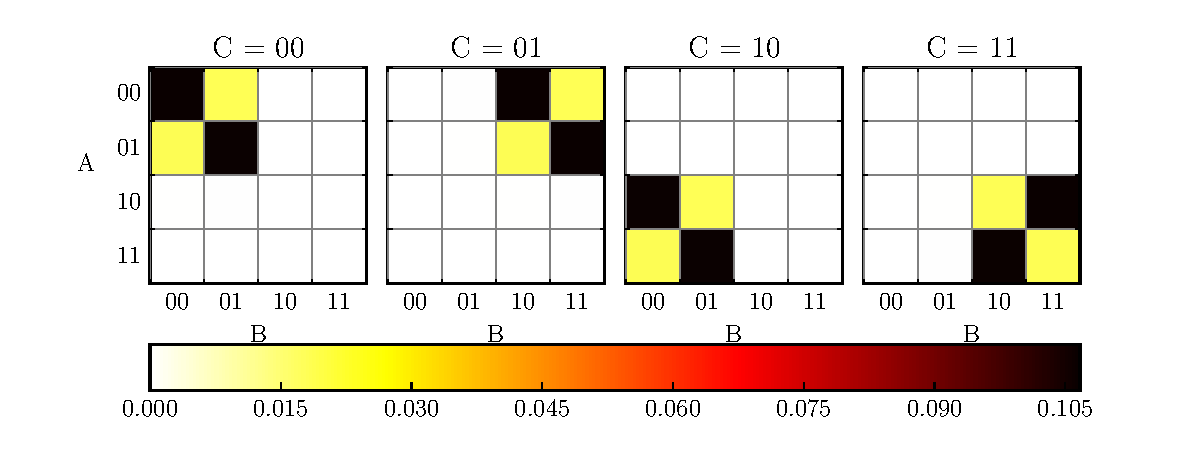
\includegraphics[scale=0.6]{../../figures/distributions/fritz_dist_plot_bits_no_title.pdf}
            \caption{The Fritz distribution visualized using a $4 \times 4 \times 4$ grid. The $4$ outcomes of $A,B,C$ are written in binary as a doublet of bits to illustrate that certain bits act as measurement pseudo-settings.}
            \label{fig:fritz_distribution_visualized}
    \end{center}
    \end{figure}
    Consequently, it is possible to define the correlation between right-bits of $A$ and $B$,
    \[ \ba{\p A_r \p B_r} = \prob[\p A_r \p B_r][00] + \prob[\p A_r \p B_r][11] - \prob[\p A_r \p B_r][01] - \prob[\p A_r \p B_r][10] \]
    And also define a CHSH inequality~\cite{CHSH_Original} for the right-bits of $A$ and $B$,
    \[ \ba{\p A_r \p B_r|\p C = 00} + \ba{\p A_r \p B_r|\p C = 01} + \ba{\p A_r \p B_r|\p C = 10} - \ba{\p A_r \p B_r|\p C = 11} \leq 2 \eq \label{eq:CHSH} \]
    Substitution of \cref{eq:fritz_dist} into \cref{eq:CHSH} yields maximal violation~\cite{Cirelson_1980},
    \[ 3 \br{\f{1}{\sqrt{2}}} - \br{-\f{1}{\sqrt{2}}} = 2\sqrt{2} \not \leq 2 \]
    The Fritz distribution $\prob[\fritz]$ can be realized as a set of quantum states and measurements. The shared resource between $A$ and $B$ (graphically denoted $\la$) is the maximally entangled Bell state:
    \[ \ket{\Phi^+} = \f{1}{\sqrt{2}}\br{\ket{00} + \ket{11}} \qquad \rho_{AB} = \ket{\Phi^+}\bra{\Phi^+} \]
    While the states shared with $C$ are the following mixed states:
    \[ \rho_{BC} = \rho_{CA} = \f{\ket{00}\bra{00} + \ket{11}\bra{11}}{2} \]
    The measurements employed by $A,B$ and $C$ are separable, projective measurements,
    \begin{align*}
        M_{A} &= \bc{\ket{0\psi_{1}}\bra{0\psi_{1}}, \ket{0\psi_{5}}\bra{0\psi_{5}}, \ket{1\psi_{3}}\bra{1\psi_{3}}, \ket{1\psi_{7}}\bra{1\psi_{7}}} \\
        M_{B} &= \bc{\ket{\psi_{6}0}\bra{\psi_{6}0}, \ket{\psi_{2}0}\bra{\psi_{2}0}, \ket{\psi_{0}1}\bra{\psi_{0}1}, \ket{\psi_{4}1}\bra{\psi_{4}1}} \\
        M_{C} &= \bc{\ket{00}\bra{00}, \ket{10}\bra{10}, \ket{01}\bra{01}, \ket{11}\bra{11}}
    \end{align*}
    Where $\ket{\psi_n}$ is shorthand for,
    \[ \ket{\psi_n} = \f{1}{\sqrt{2}}\br{\ket{0} + e^{in/4}\ket{1}} \]

    Before continuing it is worth noting that \cref{eq:fritz_dist} is non-unique. Any distribution that is equal to \cref{eq:fritz_dist} via a permutation of outcomes or exchange of parties is should also be referred to as a Fritz distribution. Moreover, the quantum realization presented here is not unique either. Nonetheless for concreteness, \cref{eq:fritz_dist} is taken as \textit{the} Fritz distribution throughout this paper.

    Additionally, it is important to understand the domain in which Fritz's proof of incompatibility is valid. Specifically, \cref{eq:CHSH} can only be applied to the triangle scenario where there exists perfect correlation between $\p C$'s outcomes and the measurement pseudo-settings (left-bits) of $\p A$ and $\p B$. The details of this restriction are discussed and proven in Fritz's original work~\cite{Fritz_2012}. As such, the incompatibility proof employed by Fritz is not applicable to any distribution that significantly deviates from the Fritz distribution presented above. For example, if one affinely combines \cref{eq:fritz_dist} with uniform noise, at what point does the resultant distribution become compatibility? This problem is discussed more in \cref{sec:noise}.

    Upon reflection, the Fritz distribution can rightly be considered slightly manufactured. The phenomenology associated with Bell non-locality or Bell incompatibility are well understood; examining these distributions under a triangle scenario embedding offers no additional perspective onto the types of resources made accessible by quantum mechanics. Therefore, it is desirable to find incompatible quantum distributions that are qualitatively different than those previously considered for the Bell scenario. In~\cite{Fritz_2012}, Fritz presented the following problem: \textit{Find an example of non-classical quantum correlations in the triangle scenario together with a proof of its non-classicality which does not hinge on Bell’s Theorem.}\footnote{In the way Fritz defines, \textit{non-classical} correlations are the class of \textit{incompatible} correlations.} The problem is understandably stated ambiguously as it is not yet entirely clear how to distinguish between non-classical distributions on differing causal structures. To refine the discussions, consider the following refinements of the problem:
    \begin{enumerate}
        \item Find proofs of causal incompatibility of quantum distributions on the triangle scenario that are not reliant on perfect correlations.
        \item Find incompatible quantum distributions on the triangle scenario that are \textit{more incompatible} that all Fritz-type embeddings.
    \end{enumerate}
    \todo[TC]{Discuss the accomplishments of this paper towards answering these problems. }

    \section{Inflation Technique}
    \begin{itemize}
        \item \todo[TC]{Summarize inflation technique}
        \item \todo[TC]{Inflations of Triangle Scenario}
        \item \todo[TC]{Demonstrate that one can derive causal incompatibility inequalities from inflation}
        \item \todo[TC]{Pre-injectable sets for Large inflation}
    \end{itemize}

    \section{Deriving Inequalities}
    \begin{itemize}
        \item \todo[TC]{Marginal problem}
        \item \todo[TC]{Popular methods: Fourier Motzkin (Convex hull, Polytope projection), Hardy implication inequalities, linear program/certificate}
        \item \todo[TC]{Overview incidence for Large Inflation}
        \item \todo[TC]{Rule out expensive methods like FM}
        \item \todo[TC]{Present some of the inequalities found}
    \end{itemize}

    \subsection{Symmetric Inequalities}
    \begin{itemize}
        \item \todo[TC]{Discuss symmetries and why they are useful}
        \item \todo[TC]{Symmetrizing Incidence Matrix}
        \item \todo[TC]{Large inflation incidence contracted drastically}
        \item \todo[TC]{Present some of the inequalities found}
    \end{itemize}

    \section{Violations}
    \begin{itemize}
        \item \todo[TC]{Fritz Distribution violates found inequalities}
    \end{itemize}
    \subsection{Numerical Optimizations}
    \begin{itemize}
        \item \todo[TC]{Generic idea}
        \item \todo[TC]{Optimization techniques used}
    \end{itemize}
    \begin{figure}
    \begin{center}
            \scalebox{1.0}{\begin{tikzpicture}[scale=1]
    \begin{scope}[every node/.style=observed]
        \node (C) at (-2, 0) {$M_C$};
        \node (B) at (2, 0) {$M_B$};
        \node (A) at (0, {2*sqrt(3)}) {$M_A$};
    \end{scope}
    \begin{scope}[every node/.style=latent]
        \node (X) at (-1, {sqrt(3)}) {$\rho_{CA}$};
        \node (Y) at (1, {sqrt(3)}) {$\rho_{AB}$};
        \node (Z) at (0, 0) {$\rho_{BC}$};
    \end{scope}
    \begin{scope}[every path/.style={draw=cause, thick}]
        \path[postaction={on each segment={mid arrow}}]
        (X) -- (A)
        (X) -- (C)
        (Y) -- (A)
        (Y) -- (B)
        (Z) -- (B)
        (Z) -- (C);
    \end{scope}
\end{tikzpicture}}
            \caption{The triangle scenario as modeled by quantum states and measurements.}
            \label{fig:triangle_scenario_quantum_model}
    \end{center}
    \end{figure}
    \subsection{Parameterizing Quantum Distributions}
    \label{sec:param_quantum_dist}
    In search of new, incompatible, quantum distributions that can be realized on the triangle scenario, numerical optimizations over the the space of quantum-accessible probability distributions are performed. To do so, we are interested in a parameterization all distributions that can be expressed as follows:
    \[ \prob[\p{ABC}]\br{abc} = \Tr\bs{\netperm^\intercal \rho_{\p{AB}}\otimes\rho_{\p{BC}}\otimes\rho_{\p{CA}} \netperm M_{\p{A},a}\otimes M_{\p{B},b} \otimes M_{\p{C},c}} \eq \label{eq:quantum_model_triangle}\]
    Where $\rho_{\p{AB}}, \rho_{\p{BC}}, \rho_{\p{CA}}$ are bipartite density matrices, $M_{\p{A}}, M_{\p{B}}, M_{\p{C}}$ are generic measurements sets and $\netperm$ is a permutation matrix that aligns the states and measurements appropriately\footnote{$\netperm$ is discussed more thoroughly in \cref{sec:perm_matrix}.}.

    In order to qualify the scope of \cref{eq:quantum_model_triangle} and associated computational complexity of the parameterization, there are a two restrictions that are made with justification. The states $\rho$ are taken to be bipartite \textit{qubit} states acting on $\s{H}^{2} \otimes \s{H}^{2}$. This is motivated by \cref{sec:fritz_distribution} in which the Fritz distribution only requires qubit states. In generality, one could consider $n$-dimensional states acting on $\s{H}^{n} \otimes \s{H}^{n}$. However, in such cases the joint density matrix $\rho_{\p{AB}}\otimes\rho_{\p{BC}}\otimes\rho_{\p{CA}}$ then acts on $\br{\Hilb^{n}}^{\otimes 6}$ requiring a $n^6 \times n^6$ matrix with $n^{12}$ entries. Therefore, $n = 2$ is far more computationally feasible than $n > 2$. Additionally, restrict our focus to projective-valued measures (PVMs) instead of projective-operator valued measures (POVMs) for three reasons. First, \cref{sec:fritz_distribution} demonstrates that PVMs are sufficient for witnessing incompatible quantum distributions in the triangle scenario. Second, generating $k$-outcome POVM measurements is possible using rejection sampling techniques~\cite{Petz_2015}, however a valid, unbiased parameterization was not found for $k > 2$. Finally, PVMs provide considerable computational advantage over POVMs as they permit \cref{eq:quantum_model_triangle} to be re-written as follows:
    \[ \prob[\p{ABC}]\br{abc} = \bramidket{m_{\p{A},a}m_{\p{B},b}m_{\p{C},c}}{\netperm^\intercal \rho_{AB}\otimes\rho_{BC}\otimes\rho_{CA} \netperm}{m_{\p{A},a}m_{\p{B},b}m_{\p{C},c}} \eq \label{eq:quantum_model_triangle_pvms}\]

    In order to parameterize all such distributions, we elect to parameterize the states and measurements separately. Although there are numerous techniques that can used when parameterizing quantum states and measurements~\cite{Petz_2015, Hedemann_2013,Fujii_2005,James_2001,Grasmair_2014,Neilsen_Chaung_2011}, a single technique is presented that was found to be most computationally suitable for our purposes.
    \subsubsection{Unitary Group}
    \label{sec:unitary_group}
    To facilitate the parameterization of quantum states states and PVMs, a parameterization of the unitary group of dimension $d$ (denoted $\s{U}\br{d}$) by Spengler, Huber and Hiesmayr~\cite{Spengler_2010_Unitary} is introduced. Discussions of its application to states and measurements are deferred to \cref{sec:states} and \cref{sec:measurements} respectively.

    In Ref.~\cite{Spengler_2010_Unitary}, Spengler \textit{et. al.} proved that all unitaries $U \in \s{U}\br{d}$ can be parameterized without degeneracy as follows:
    \[ U = \bs{\prod_{m=1}^{d-1} \br{\prod_{n=m+1}^{d} \exp\br{i P_n \lambda_{n,m}}\exp\br{i \si_{m,n} \lambda_{m,n}}}} \tcdot \bs{\prod_{l=1}^{d} \exp\br{iP_l \lambda_{l,l}}}  \eq \label{eq:spengler_unitary} \]
    Where $\la = \bc{\la_{n,m} \mid n,m \in 1, \ldots, d}$ form a $d \times d$ matrix of real-valued parameters with periodicities $\la_{m,n} \in \bs{0, \f{\pi}{2}}$ for $m < n$ and $\la_{m,n} \in \bs{0, 2 \pi}$ for $m \geq n$.
    \[ \la = \begin{pmatrix}
        \la_{1,1} & \cdots & \la_{1, d} \\
        \vdots & \ddots & \vdots \\
        \la_{d,1} & \cdots & \la_{d, d} \\
    \end{pmatrix} \]
    And where $P_l$ are one-dimensional projective operators,
    \[ P_l = \ket{l}\bra{l} \qquad 1 \leq l \leq d \eq \label{eq:projective_operator} \]
    and the $\si_{m,n}$ are generalized anti-symmetric $\si$-matrices,
    \[ \sigma_{m,n} = -i \ket{m}\bra{n} +i \ket{n}\bra{m} \qquad 1 \leq m < n \leq d\]
    The SSH parameterization (\cref{eq:spengler_unitary}) is unique in that each of the real-valued parameters $\la_{n,m}$ has physical significance. For the sake of reference, let us label the matrix exponential terms in \cref{eq:spengler_unitary} in a manner that corresponds to their affect on an orthonormal basis $\bc{\ket{1}, \ldots, \ket{d}}$.
    \begin{align*}
    \begin{split}
        GP_l &= \exp\br{iP_l \lambda_{l,l}} \\
        RP_{n,m} &= \exp\br{i P_n \lambda_{n,m}} \\
        R_{m,n} &= \exp\br{i \si_{m,n} \lambda_{m,n}}
    \end{split} \eq \label{eq:exp_terms}
    \end{align*}
    For example, $R_{m,n} = \exp\br{i \si_{m,n} \lambda_{m,n}}$ applies a rotation to the sub-space spanned by $\ket{m}$ and $\ket{n}$ for $m < n$. Analogously, $RP_{n,m}$ generates the relative phase between $\ket{m}$ and $\ket{n}$ for $m > n$ and $GP_l$ fixes the global phase of $\ket{l}$. Possessing a parameterization that maintains this physical interpretation is useful as it allows one to readily eliminate any degeneracies. For the purposes of quantum distributions such as \cref{eq:quantum_model_triangle}, it should be clear that any contributions to global phase are irrelevant. The SSH parameterization becomes especially attractive because it readily permits one to drop the global phase terms by setting $\la_{l,l} = 0$ for all $l = 1, \ldots, d$. It is convenient to denote the set of all unitaries up to global phase considerations as $\ti {\s{U}}\br{d}$ and express $\ti {U} \in \ti {\s{U}}\br{d}$ using $d\br{d-1}$ real-valued parameters:
    \[ \ti U = \prod_{m=1}^{d-1} \br{\prod_{n=m+1}^{d} RP_{n,m}R_{m,n}} \eq \label{eq:spengler_unitary_gp} \]
    Another attractive feature of the SSH parameterization not mentioned in~\cite{Spengler_2010_Unitary} is that \cref{eq:spengler_unitary}, and thus \cref{eq:spengler_unitary_gp}, can be implemented in a computationally efficient manner. This is discussed in \cref{sec:comp_spengler}.
    \subsubsection{Measurements}
    \label{sec:measurements}
    For each measurement set $M$ in \cref{eq:quantum_model_triangle}, we consider a $d$-element projective-valued measure (PVM) $M = \bc{M_1, \ldots, M_d}$ satisfying a number of familiar constraints:
    \begin{gather*}
    \forall \ket{\phi} \in \Hilb^d: \bra{\phi} M_i \ket{\phi} \geq 0 \qquad \sum_{i=1}^{d} M_i = \ident_{d} \\
    M_i = \ket{m_i}\bra{m_i} \qquad M_i M_j = \de_{ij} M_i
    \end{gather*}
    Therefore, parameterizing $M$ corresponds to parameterizing the set of all orthonormal basis $\bc{\ket{\psi_1}, \ldots, \ket{\psi_d}}$ of $\Hilb^d$.
    First note that any such basis can be transformed into the computational basis $\bc{\ket{1}, \ldots, \ket{d}}$ by a unitary denoted $U^{-1} \in \mathcal{U}\br{d}$.
    \[ \forall i : U^{-1} \ket{\psi_i} = \ket{i} \eq \label{eq:unitary_transform}\]
    With this observation, all that is required is to parameterize the set of all unitaries $U \in \mathcal{U}\br{d}$. Specifically, the projective property each $M_i \in M$ means that the global phase of $U$ is completely arbitrary; one only needs to consider parameterizing unitaries up to global phase using \cref{eq:spengler_unitary_gp}.
    \[ M = \bc{\ti U \ket{i} \bra{i} \ti U^{\dagger} \mid i \in \bc{1, \ldots, d}} \]
    For the purposes discussed in \cref{sec:param_quantum_dist}, only $d = 4$ outcome measurements are utilized and therefore requiring $4\br{4 - 1} = 12$ real-valued parameters. This method was inspired by the measurement seeding method of P{\'{a}}l and V{\'{e}}rtesi's~\cite{Pal_2010} iterative optimization technique.
    \subsubsection{States}
    \label{sec:states}

    Each state $\rho \in \br{\rho_{AB}, \rho_{BC}, \rho_{CA}}$ of \cref{eq:quantum_model_triangle} is modeled as a two-qubit density matrices acting on $\Hilb^2 \otimes \Hilb^2$. The space of all such states corresponds to the space of all $4\times 4$ positive semi-definite hermitian matrices with unitary trace.
    \[ \forall \ket{\phi} \in \Hilb^d: \bra{\phi} \rho \ket{\phi} \geq 0 \qquad \rho^{\dagger} = \rho \qquad \Tr\br{\rho} = 1 \eq \label{eq:density_matrix}\]
    Although is common to parameterize all such matrices using a Cholesky decomposition~\cite{Grasmair_2014}, we make use of the non-degenerate SHH parameterization~\cite{Spengler_2010_Unitary} and the spectral decomposition of $\rho$. Retaining full generality, consider full-rank density matrices:
    \[ \rho = \sum_{i=1}^{d} p_i \ket{\psi_i}\bra{\psi_i} \qquad \sum_{i=1}^{d} p_i = 1, p_i \geq 0 \eq \label{eq:param_density} \]
    Where $\bc{p_i}$ are the eigenvalues of $\rho$ and $\bc{\ket{\psi_i}}$ are its eigenstates. It is here that one recognizes the reapplication of \cref{eq:unitary_transform}: any orthonormal basis $\bc{\ket{\psi_i}}$ of $\Hilb^d$ can be transformed into a computational basis $\bc{\ket{i}}$ by a unitary transformation $U \in \mathcal{U}\br{d}$ such that $\ket{\psi_i} = U\ket{i}$. Analogous to the projective measurements considered in \cref{sec:measurements}, the global phase contributions are redundant.
    \[ \rho = \sum_{i=1}^{d} p_i \ti U\ket{i}\bra{i} \ti U^{\dagger} \]
    Parameterizing the eigenvalues requires $d - 1$ real-valued parameters due to the trace constraint of \cref{eq:density_matrix}. The eigenvalues are parameterized without degeneracy using a tuple of $d-1$ parameters $\lambda = \br{\lambda_1, \ldots, \lambda_{d-1}}, \lambda_i \in \bs{0, 2 \pi}$ using hyperspherical coordinates~\cite{Hedemann_2013, Spengler_2010_Unitary}:
    \begin{align*}
    \eq \label{eq:convex_param}
    \begin{split}
        p_n &= \prod_{i=1}^{n-1} \sin^2 \lambda_i \\
        p_j &= \cos^2 \lambda_j \prod_{i=1}^{j-1} \sin^2 \lambda_i \quad \forall j \in 1, \ldots, n - 1
    \end{split}
    \end{align*}
    Therefore it is possible to parametrize all $d$-dimensional density matrices satisfying \cref{eq:density_matrix} using $d\br{d - 1} + d - 1 = d^2 -1$ parameters.
    \subsubsection{Permutation Matrix}
    \label{sec:perm_matrix}
    \begin{figure}
        \centering
        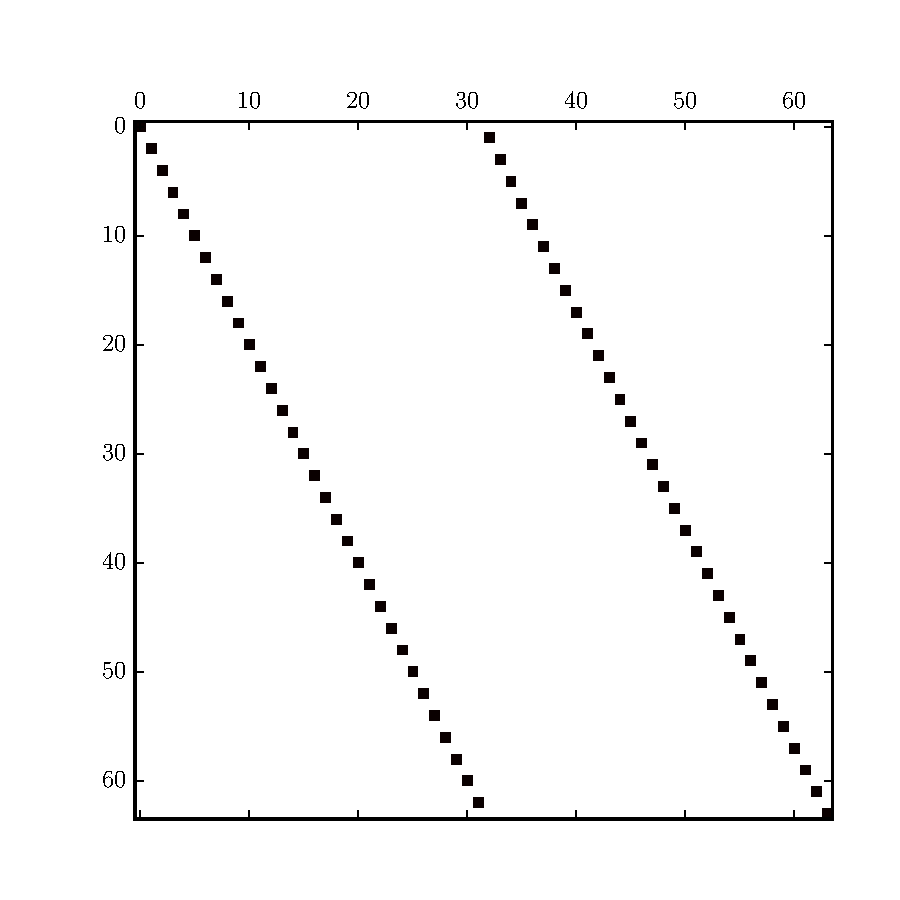
\includegraphics[trim={1cm 1.2cm 1.0cm 1cm},clip,width=0.4\textwidth]{../../figures/perm_mtrx.pdf}
        \caption{The triangle scenario permutation matrix $\netperm$ for $\br{\Hilb^2}^{\otimes 6}$. Black represents a value of $1$ and white represents $0$.}
        \label{fig:perm_mtrx}
    \end{figure}
    Finally, we introduce the a permutation matrix $\netperm$ for the triangle scenario. For bipartite qubit states, $\netperm$ is the $64\times64$ bit-wise matrix depicted in \cref{fig:perm_mtrx}. Upon examination of \cref{eq:quantum_model_triangle_pvms}, we consider $\netperm$ to be acting on the joint global state $\rho_{\p{AB}} \otimes \rho_{\p{BC}} \otimes \rho_{\p{CA}}$. To illuminate its necessity, consider \cref{eq:quantum_model_triangle} in the absence of $\netperm$.
    \begin{align*}
    \prob[\p{ABC}]\br{abc} &\stackrel{?}{=} \Tr\bs{\br{\rho_{\p{AB}} \otimes \rho_{\p{BC}} \otimes \rho_{\p{CA}}} \br{M^a_{\p{A}}\otimes M^b_{\p{B}} \otimes M^c_{\p{C}}}}\\
    &= \Tr\bs{\br{\rho_{\p{AB}}M^a_{\p{A}}}\otimes\br{\rho_{\p{BC}}M^b_{\p{B}}}\otimes\br{\rho_{\p{CA}}M^c_{\p{C}}}}\\
    &= \Tr\br{\rho_{\p{AB}}M^a_{\p{A}}}\Tr\br{\rho_{\p{BC}}M^b_{\p{B}}}\Tr\br{\rho_{\p{CA}}M^c_{\p{C}}}\\
    &= \prob[\p{A}\mid \rho_{\p{AB}}]\br{a}\prob[\p{B}\mid \rho_{\p{BC}}]\br{b}\prob[\p{C}\mid \rho_{\p{CA}}]\br{c}
    \end{align*}
    On an operational level, this corresponds to $A$ making a measurement on \textit{both} subsystems of $\rho_{AB}$ and \textit{not} on any component of $\rho_{CA}$. This is analogously troubling for $B$ and $C$ as well. To resolve this issue, the permutation matrix $\netperm$ corresponds to \textit{aligning} the underlying $6$-qubit joint state $\rho$ with the joint measurement $M$. To understand its effect, consider its effect on $6$-qubit pure state $\ket{q_1} \otimes \cdots \otimes \ket{q_6} = \ket{q_1q_2q_3q_4q_5q_6}$ where $\forall i : \ket{q_i} \in \Hilb^2$.
    \[ \netperm\ket{q_1q_2q_3q_4q_5q_6} = \ket{q_2q_3q_4q_5q_6q_1} \]
    $\netperm$ acts as a \textit{partial transpose} on $\br{\Hilb^2}^{\otimes 6}$ by shifting the underlying tensor structure one subsystem to the ``left''. It is uniquely defined by its action on all $2^6$ orthonormal basis elements of $\br{\Hilb^2}^{\otimes 6}$,
    \[ \netperm \defined \sum_{\ket{q_i} \in \bc{\ket{0}, \ket{1}}}\ket{q_2q_3q_4q_5q_6q_1}\bra{q_1q_2q_3q_4q_5q_6} \]
    \subsection{Results}
    \begin{itemize}
        \item \todo[TC]{Plots of various optimizations}
        \item \todo[TC]{Features of maximally violating distributions}
    \end{itemize}

    \section{Noise}
    \label{sec:noise}
    \begin{itemize}
        \item \todo[TC]{Recall why noise is important (experimental and foundational)}
        \item \todo[TC]{Describe our noise model}
        \item \todo[TC]{Plots}
        \item \todo[TC]{Define and discuss the crossing point}
        \item \todo[TC]{Discussion as to what noise measures}
    \end{itemize}

    \section{Conclusions}
    \begin{itemize}
        \item \todo[TC]{Inflation technique capable of finding inequalities witnessing quantum/classic difference in TS}
        \item \todo[TC]{Causal incompatibility inequalities found violated by known distributions}
        \item \todo[TC]{Maximal distributions are different than Fritz but still rely on Bell's theorem}
        \item \todo[TC]{Refinement on Fritz's question}
    \end{itemize}

    \section*{Acknowledgments}
    \begin{itemize}
        \item \todo[TC]{Elie}
        \item \todo[TC]{Perimeter}
        \item \todo[TC]{University of Waterloo}
        \item \todo[TC]{Possible due to Mike Lazaridis Scholarship}
    \end{itemize}
    \appendix
    \section{Computationally Efficient Parameterization of the Unitary Group}
    \label{sec:comp_spengler}

    If \cref{sec:unitary_group}, the SSH parameterization was introduced as a non-degenerate parameterization of the unitary group $\s{U}\br{d}$. As presented, the SSH parameterization suffers due to the presence of computationally expensive matrix exponential terms~\cite{Moler_2003}. Although not explicitly mentioned in~\cite{Spengler_2010_Unitary}, it is possible to remove the reliance on matrix exponential operations in \cref{eq:spengler_unitary} by utilizing the explicit form of the exponential terms in \cref{eq:exp_terms}. As a first step, recognize the defining property of the projective operators \cref{eq:projective_operator},
    \[ P_l^k = \br{\ket{l}\bra{l}}^k = \ket{l}\bra{l} = P_l \]
    This greatly simplifies the global phase terms $GP_l$,
    \[ GP_l = \exp\br{iP_l \lambda_{l,l}} = \sum_{k=0}^{\inf} \f{\br{iP_l \lambda_{l,l}}^k}{k!} = \ident + \sum_{k=1}^{\inf} \f{\br{i \lambda_{l,l}}^k}{k!}P_l^k = \ident + P_l \bs{\sum_{k=1}^{\inf} \f{\br{i \lambda_{l,l}}^k}{k!}} = \ident + P_l \br{e^{i \lambda_{l,l}} - 1} \eq \label{eq:unitary_GP} \]
    Analogously for the relative phase terms $RP_{n,m}$,
    \[ RP_{n,m} = \cdots = \ident + P_n \br{e^{i \lambda_{n,m}} - 1} \eq \label{eq:unitary_RP} \]
    Finally, the rotation terms $R_{m,n}$ can also be simplified by examining powers of $i \sigma_{n,m}$,
    \[ R_{m,n} = \exp\br{i \si_{m,n} \lambda_{m,n}} = \sum_{k=0}^{\inf} \f{\br{\ket{m}\bra{n} - \ket{n}\bra{m}}^k \lambda_{m,n}^k}{k!} \]
    One can verify that the following properties hold,
    \begin{align*}
        \br{\ket{m}\bra{n} - \ket{n}\bra{m}}^0 &= \ident \\
        \forall k \in \N, k \neq 0 : \br{\ket{m}\bra{n} - \ket{n}\bra{m}}^{2k} &= \br{-1}^k\br{\ket{m}\bra{m} + \ket{n}\bra{n}} \\
        \forall k \in \N : \br{\ket{m}\bra{n} - \ket{n}\bra{m}}^{2k+1} &= \br{-1}^k\br{\ket{m}\bra{n} - \ket{n}\bra{m}}
    \end{align*}
    Revealing the simplified form of $R_{m,n}$,
    \[ R_{m,n} = \ident + \br{\ket{m}\bra{m} + \ket{n}\bra{n}} \sum_{j=1}^{\inf} \br{-1}^j\f{\lambda_{n,m}^{2j}}{\br{2j}!} + \br{\ket{m}\bra{n} - \ket{n}\bra{m}} \sum_{j=0}^{\inf} \br{-1}^j\f{\lambda_{n,m}^{2j+1}}{\br{2j+1}!} \]
    \[ R_{m,n} = \ident + \br{\ket{m}\bra{m} + \ket{n}\bra{n}} \br{\cos\lambda_{n,m} - 1} + \br{\ket{m}\bra{n} - \ket{n}\bra{m}} \sin\lambda_{n,m} \eq \label{eq:unitary_R} \]
    By combining the optimizations of \cref{eq:unitary_GP,eq:unitary_RP,eq:unitary_R} together we arrive at an equivalent form for \cref{eq:spengler_unitary} that is computational more efficient.
    \[ U = \bs{\prod_{m=1}^{d-1} \br{\prod_{n=m+1}^{d} R_{m,n}RP_{n,m}}} \tcdot \bs{\prod_{l=1}^{d} GP_{l}}  \eq \label{eq:spengler_unitary_fast} \]

    \bibliography{../references}
\end{document}